%% SW arkitektur: Implementation View

Inden programmerne designes, fastlægges en struktur for kildekoden. På den måde er det nemmere for flere programmører at arbejde med delene i programmet samtidigt.

Strukturen skal være som vist i figur \ref{fig:implementationview}. Under mappen ''Kildekode'' skal hver klasse have en mappe med dertil hørende filer. Ligeledes med ''Testprogrammer'' mappen, som indholder testprogrammer som verificerer funktionaliteten af de enkelte moduler.
Mappen ''Kompilerede programmer'' er til de endelige programmer.

\begin{figure}[htbp] \centering
{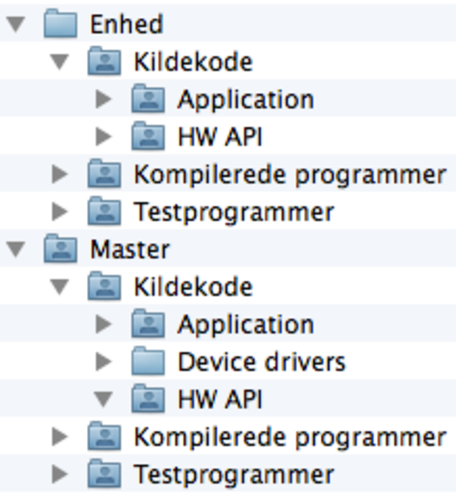
\includegraphics[scale=0.7]{filer/pics/SW-Implementation-View}}
\caption{Mappestruktur for software-kilder}
\label{fig:implementationview}
\end{figure}